%%%%%%%%%%%%%%%%%%%%%%%%%%%%%%%%%%%%%%%%%%%%%%%%%%%%%%%%%%%%%%%%
%\section{Oscillation Physics}
%\label{sec:landscape-osc}

The first positive hint for neutrino flavor-change was uncovered in the 1960's with the first measurement of the flux of neutrinos from the sun. The hint compounded in the late 1980's, with high-statistics measurements of the differential flux of muon-type neutrinos produced by the collisions of cosmic rays with the earth's atmosphere. Both hints were ultimately confirmed in the late 1990's and early 2000's by the Super-Kamiokande and SNO experiments. Concurrently, neutrino oscillations were confirmed as the dominant physics behind neutrino flavor change. 

Neutrino oscillations imply nonzero neutrino masses and flavor-mixing in the leptonic charged-current interactions.  That the neutrino masses are not zero is among the most important discoveries in fundamental particle physics of the twenty-first century. Understanding the mechanism behind nonzero neutrino masses is among the unresolved mysteries that drive particle physics today; they remain one of the few unambiguous facts that point to the existence of new particles and interactions, beyond those that make up the remarkable standard model of particle physics. Learning more about the properties of neutrinos is a very high priority for particle physics, and neutrino oscillations remain, as of today, the only phenomenon capable of observing the neutrino masses and lepton mixing in action. Precision measurements of neutrino oscillations have the potential to play a leading role in shaping particle physics in the next few decades. 

Almost all neutrino data can be understood within the three-flavor paradigm with massive neutrinos, the simplest extension of the standard model capable of reconciling theory with observations. A handful of intriguing results, including those from the LSND, MiniBooNE, and short-baseline reactor experiments, remain unexplained and are currently the subject of intense experimental and theoretical scrutiny. If confirmed as the manifestation of new physics involving neutrinos -- e.g., new neutrino states --  these will open the door to more neutrino-related questions, many of which can be further explored with DUNE. We will return to those later but assume, conservatively, that the resolutions to these so-called short-baseline anomalies lie outside of neutrino-related particle physics. 

\subsection{Oscillation Physics with Three Neutrino Flavors}

The three-flavor paradigm with massive neutrinos consists of introducing distinct, nonzero, masses for at least two neutrinos, while maintaining the remainder of the standard model of particle physics. Hence, neutrinos interact only via the standard model charged-current and neutral-current weak interactions. The neutrino mass eigenstates -- defined as $\nu_1,\nu_2, \nu_3$ with masses, $m_1, m_2, m_3$, respectively -- are distinct from the neutrino charged-current interaction eigenstates, also referred to as the flavor eigenstates -- $\nu_e$, $\nu_{\mu}$, $\nu_{\tau}$, labelled according to the respective charged-lepton $e,\mu,\tau$ to which they couple in the charged-current weak interaction. The flavor eigenstates can be expressed as linear combinations of the mass eigenstates (and vice-versa). The coefficients of the respective linear combinations define a unitary $3\times 3$ mixing matrix, referred to as the neutrino mixing matrix, the leptonic mixing matrix, or the Pontecorvo-Maki-Nakagawa-Sakata (PMNS) matrix, as follows:
\begin{equation}
\left(\begin{array}{c} \nu_e \\ \nu_{\mu} \\ \nu_{\tau} \end{array}\right) = \left(\begin{array}{ccc} U_{e1} & U_{e2} & U_{e3} \\  U_{\mu1} & U_{\mu2} & U_{\mu3}  \\  U_{\tau1} & U_{\tau2} & U_{\tau3}  \end{array}\right) \left(\begin{array}{c} \nu_1 \\ \nu_2 \\ \nu_3 \end{array}\right).
\end{equation}
The PMNS matrix is the leptonic-equivalent of the Cabibbo-Kobayashi-Maskawa (CKM) matrix that describes the charged-current interactions of quark mass eigenstates. If the neutrinos are Dirac fermions, taking advantage of the unitary nature of the matrix and the ambiguity in defining the relative phases among the standard model lepton fields, the neutrino mixing matrix, like the CKM matrix, can be unambiguously parameterized with three mixing angles and one complex phase. If, however, the neutrinos are Majorana fermions, there are fewer field-redefinitions available and one ends up with at most two other physical complex phases.\footnote{Majorana phases can also be interpreted as complex phases of the neutrino mass eigenvalues and need not be considered as part of the neutrino mixing matrix.}  Strictly speaking, these so-called Majorana phases can manifest themselves in ``neutrino--antineutrino'' oscillations \cite{deGouvea:2002gf} and could be observed in neutrino oscillation experiments. These effects, however, are expected to be unobservably small and will be henceforth ignored, along with the Majorana phases. For all practical purposes, neutrino oscillation experiments cannot distinguish Majorana from Dirac neutrinos. Majorana phases are expected to play a significant role in experiments that are sensitive to the Majorana versus Dirac nature of the neutrinos, including searches for neutrinoless double-beta decay. 

The PDG-parameterization \cite{Tanabashi:2018oca}, used throughout this report, makes use of three mixing angles $\theta_{12}$, $\theta_{13}$, and $\theta_{23}$, defined as
\begin{eqnarray}
\tan^2\theta_{12} &\equiv& \frac{|U_{e2}|^2}{|U_{e1}|}, \\
\tan^2\theta_{23} &\equiv& \frac{|U_{\mu3}|^2}{|U_{\tau3}|}, \\
\sin^2\theta_{13} &\equiv& |U_{e3}|^2,
\end{eqnarray} 
and one the complex phase $\deltacp$, defined as
\begin{equation}
\deltacp \equiv -{\rm arg}(U_{e3}).
\end{equation}
For values of $\deltacp\neq 0,\pi$, and assuming none of the $U_{\alpha i}$ vanish ($\alpha=e,\mu,\tau$, $i=1,2,3$), the neutrino mixing matrix is complex and CP-invariance is violated in the lepton sector. This, in turn, manifests itself as different oscillation probabilities, in vacuum, for neutrinos and antineutrinos: $P(\nu_{\alpha}\to\nu_{\beta})\neq P(\bar{\nu}_{\alpha}\to\bar{\nu}_{\beta})$, $\alpha,\beta=e,\mu,\tau$, $\alpha\neq\beta$.\footnote{For neutrino disappearance, in vacuum, the relation $P(\nu_{\alpha}\to\nu_{\alpha}) =P(\bar{\nu}_{\alpha}\to\bar{\nu}_{\alpha})$ is a consequence of the CPT-theorem.} 

Information on the values of the neutrino masses comes from measurements of the neutrino oscillation frequencies, which are proportional to the differences of the squares of the neutrino masses, $\Delta m^2_{ij}\equiv m_i^2-m_j^2$. Since all positive evidence for nonzero neutrino masses comes from measurements of neutrino oscillations, there is no direct information concerning the values of the masses themselves, only the mass-squared differences. As far as neutrino oscillation data are concerned, the hypothesis that the lightest neutrino mass is exactly zero is just as valid as the hypothesis that all neutrino masses are nonzero and almost degenerate. Three neutrino masses allow for two independent mass-squared differences and the existing neutrino data point to two hierarchically different $\Delta m^2$, one whose magnitude is of order $10^{-4}$~eV$^2$, the other with magnitude of order $10^{-3}$~eV$^2$. 

With this information, it is possible to unambiguously define the neutrino masses in a convenient way, as follows.\footnote{Equivalently, one can use the neutrino mixing matrix to define the neutrino mass eigenstates. $\nu_1$ could be defined as the state associated to the largest $|U_{ei}|^2$ ($i=1,2,3$), $\nu_2$ to the second largest $|U_{ei}|^2$, and $\nu_3$ to the smallest $|U_{ei}|^2$: $|U_{e1}|^2>|U_{e2}|^2>|U_{e3}|^2$.} The mass-squared difference with the smallest magnitude is defined to be $\Delta m^2_{21}$, positive-definite so $m_2^2>m_1^2$. The third mass eigenvalue is such that $|\Delta m^2_{31}|\sim|\Delta m^2_{32}|$, of order $10^{-3}$~eV$^2$ while the sign of  $\Delta m^2_{31}, \Delta m^2_{32}$ defines the neutrino mass ordering, or the neutrino mass hierarchy. If $\Delta m^2_{31}, \Delta m^2_{32}>0$, the neutrino mass ordering is defined to be `normal' and $m_1^2<m_2^2<m_3^2$. If $\Delta m^2_{31}, \Delta m^2_{32}<0$, the neutrino mass ordering is defined to be `inverted' and $m_3^2<m_1^2<m_2^2$. This definition allows one to change from a normal to an inverted ordering without having to change the relationship between the neutrino mixing matrix and the various experimental results. The distinct neutrino mass orderings are illustrated in Figure~\ref{massordering}.
\begin{dunefigure}[Mass Ordering Illustration]{massordering}{
   Fractional flavour content, $|U_{\alpha i}|^2$ ($\alpha = e, \mu, \tau$) of the three mass eigenstates $\nu_i$, based on the current best-fit values of the mixing angles. $\deltacp$ is varied from 0 (bottom of each coloured band) to $180^\circ$ (top of coloured band), for normal and inverted mass ordering on the left and right, respectively. The different colours correspond to the $\nu_e$ fraction (red), $\nu_\mu$ (green) and $\nu_\tau$ (blue). 
%   {\bf [The figure here is a placeholder.]}
}
  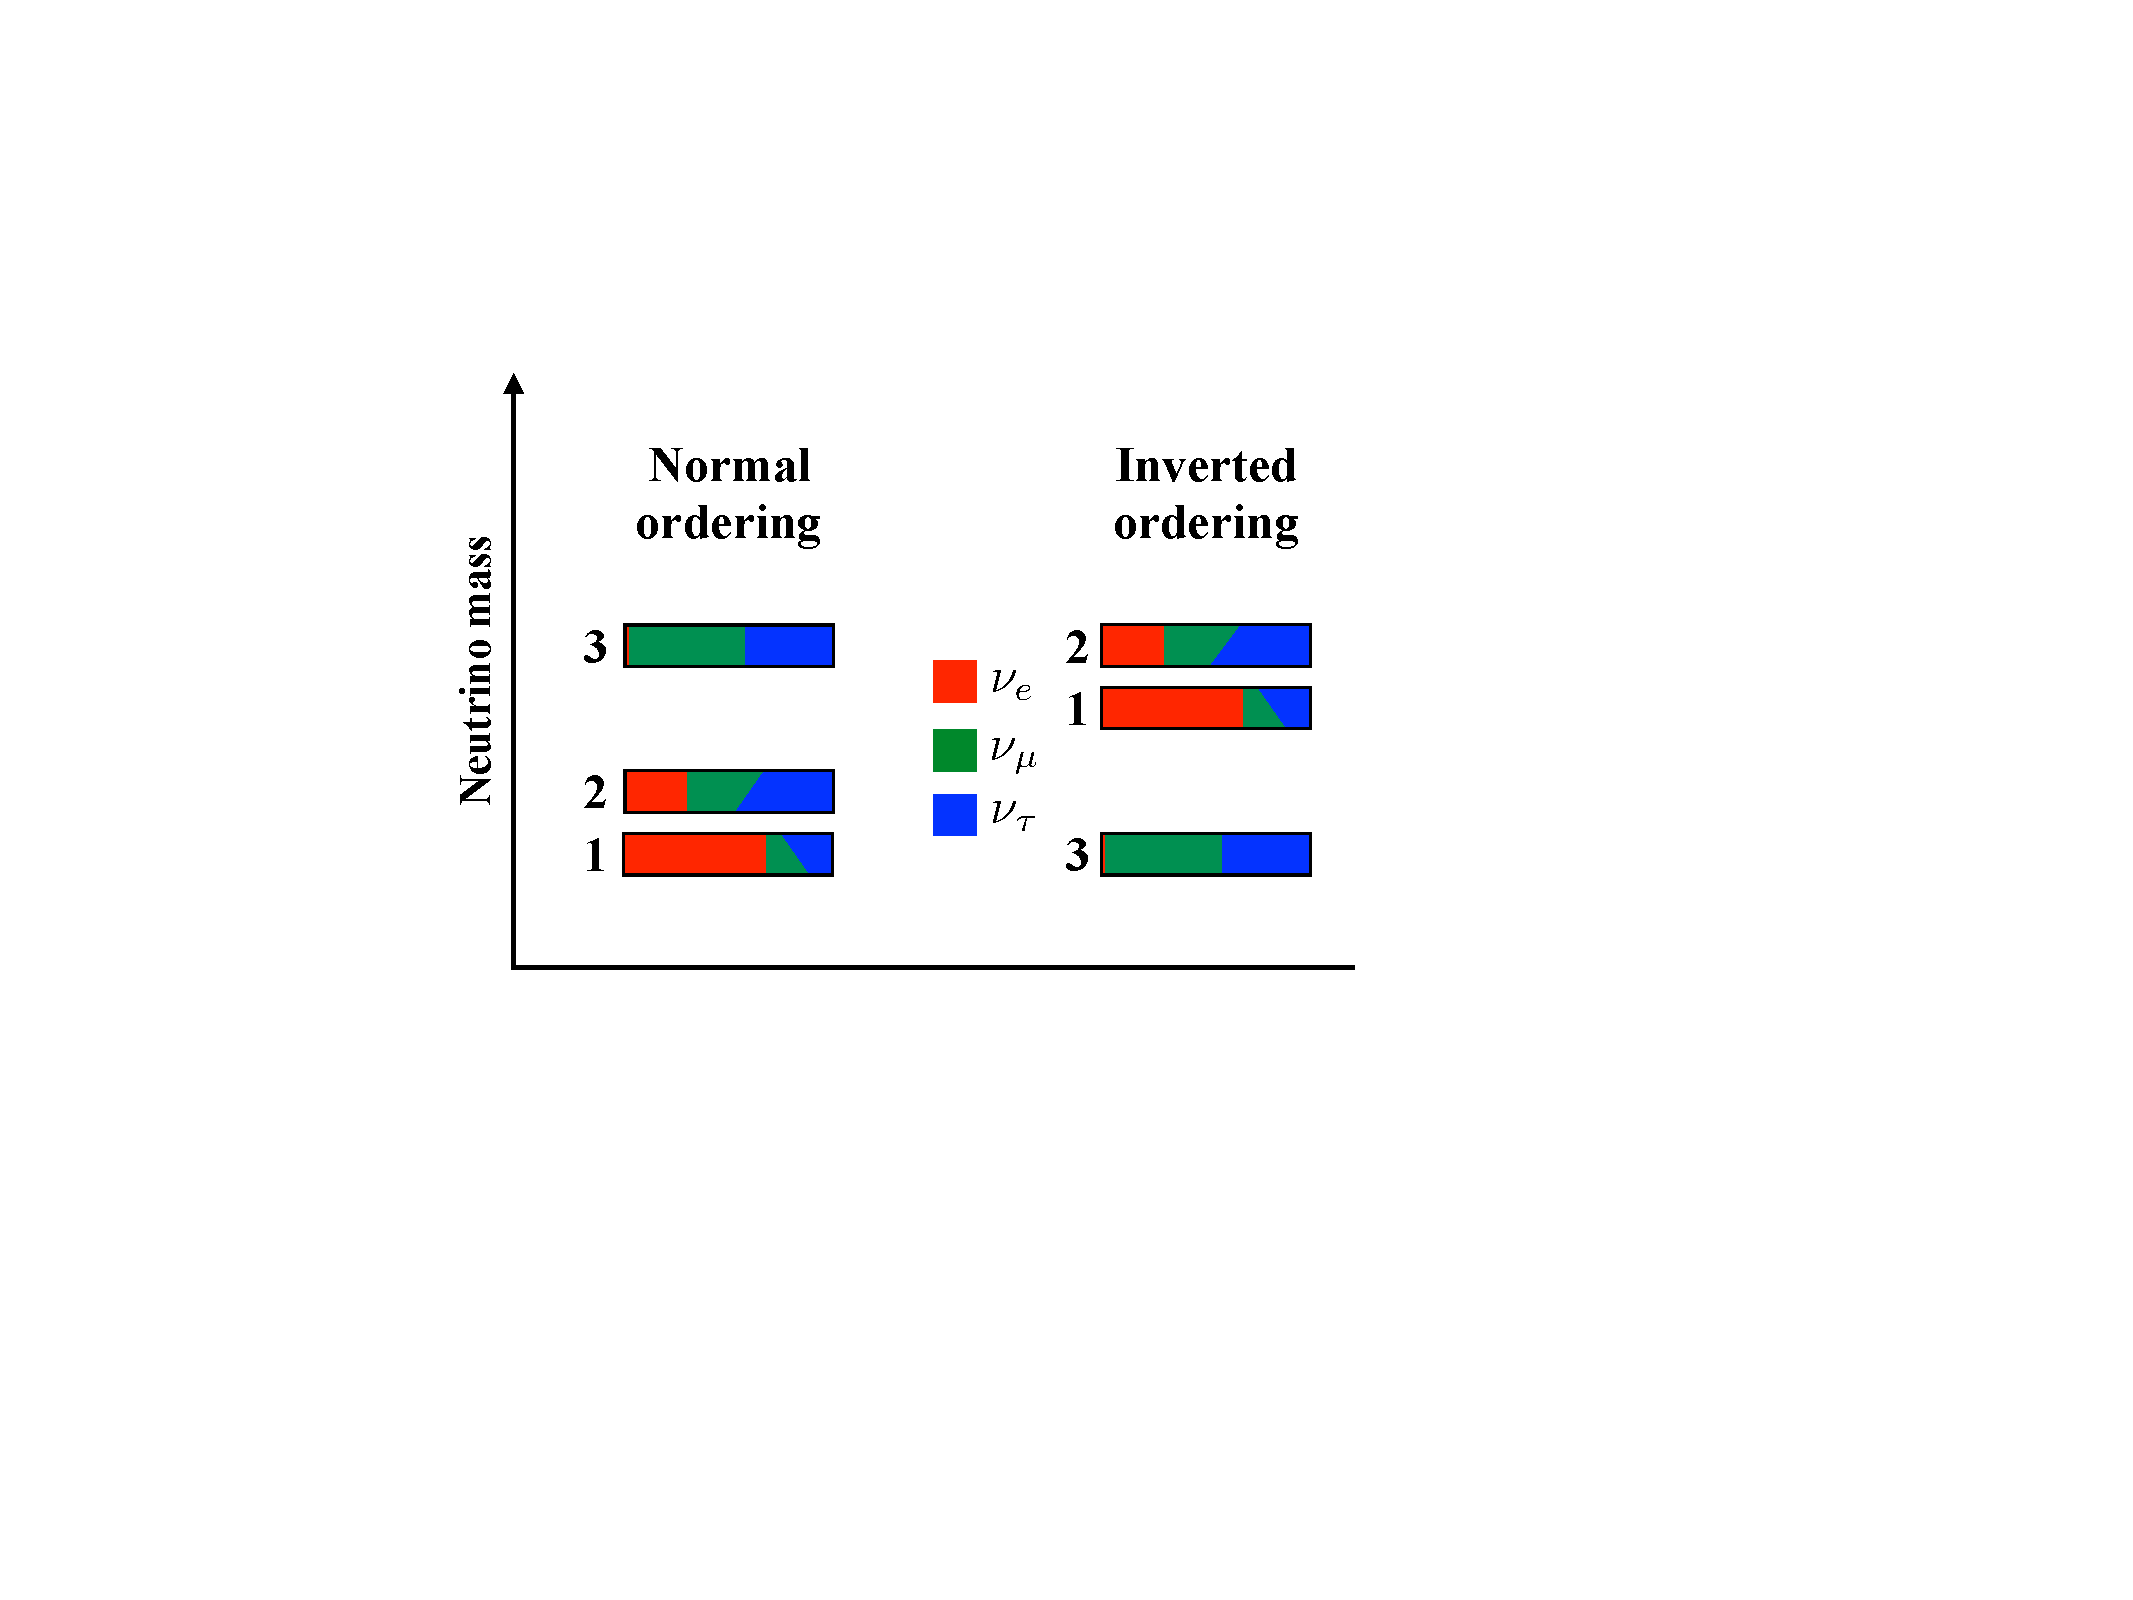
\includegraphics[width=0.6\textwidth]{graphics/PastedGraphic-1.pdf}
\end{dunefigure}

\subsubsection{Synthesis of Experimental Inputs} 

The world's neutrino data significantly constrain all of the oscillation parameters in the three-flavor paradigm. The results of a recent global fit \cite{Esteban:2018azc} to all neutrino data, except those associated to the short-baseline anomalies, are depicted in Fig.~\ref{nufit40}. The magnitudes of both mass-squared differences are known at better than 3\%, while, at the one sigma level, $\sin^2\theta_{12}$, $\sin^2\theta_{13}$, $\sin^2\theta_{23}$ are known at better than the 5\% level. Note, however, that the error bars are rather non-Gaussian, especially for $\sin^2\theta_{23}$. At the three sigma level,  according to \cite{Esteban:2018azc}, $\sin^2\theta_{23}$ is constrained to lie between 0.43 and 0.62 so values of $\sin^2\theta_{23}>0.5$ and $\sin^2\theta_{23}<0.5$ are allowed.
\begin{dunefigure}[Nufit 4.0 global fit]{nufit40}{Global three-neutrinos-oscillation analysis from \cite{Esteban:2018azc}. Each panel depicts the two-dimensional projection of the allowed six-dimensional region after marginalization with respect to the undisplayed parameters. The different contours correspond to the two-dimensional allowed regions at 1$\sigma$, 90\%, 2$\sigma$, 99\%, 3$\sigma$ CL (2~dof). Note that the top panel refers to $\Delta m^2_{31}$ in the case of the normal mass-ordering and $\Delta m^2_{32}$ in the case of the inverted one. The regions in the lower four panels are defined using $\Delta \chi^2$ relative to minimum value of $\chi^2$ obtained for a fixed choice of the mass ordering, normal ordering on the left-hand-side, inverted ordering on the right-hand-side.
}
  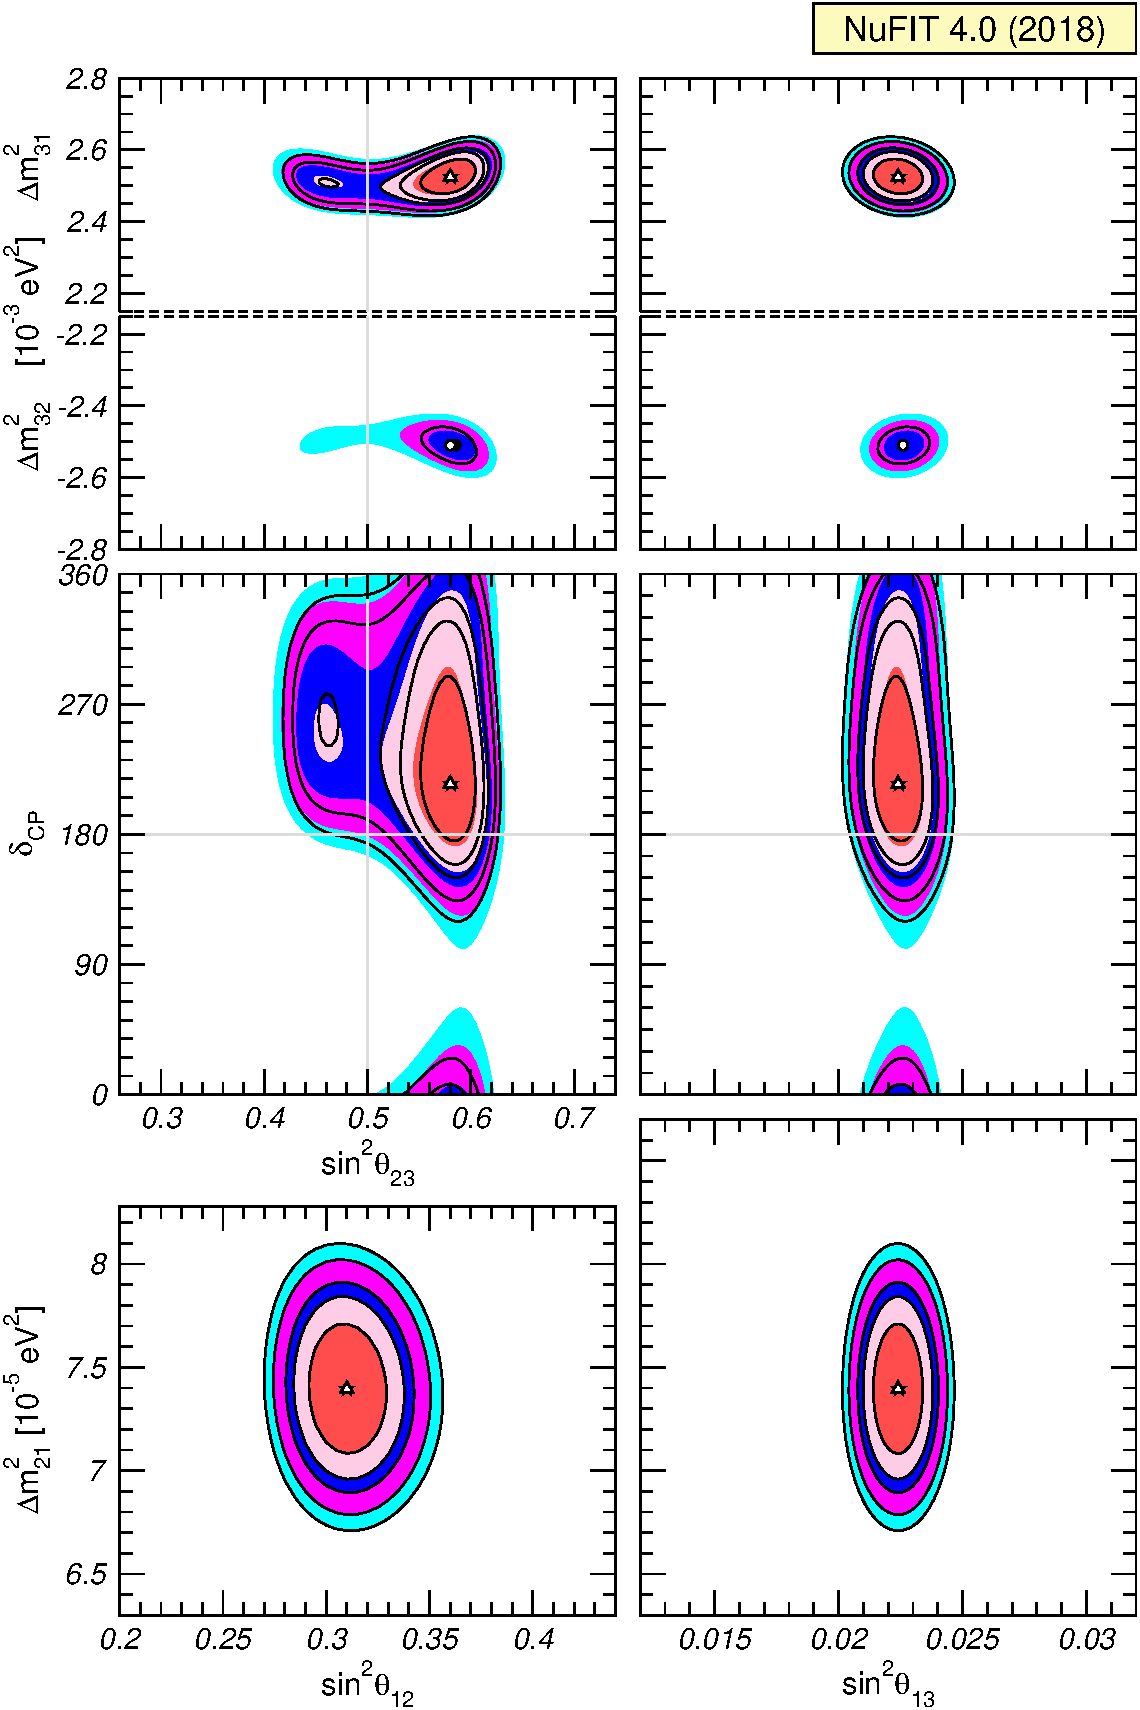
\includegraphics[width=0.7\textwidth]{nufit40_global.pdf}
\end{dunefigure}

Several open questions remain. The neutrino mass ordering is unknown. Current data prefer the normal ordering but the inverted one still provides a decent fit to the data. The octant of $\theta_{23}$ (whether $\sin^2\theta_{23}<0.5$ [$\theta_{23}<\pi/4$] or $\sin^2\theta_{23}>0.5$ [$\theta_{23}>\pi/4$]) remains unknown. The value of $\deltacp$ is only poorly constrained. While positive values of $\sin\deltacp$ are disfavored, all values between $\pi$ and $2\pi$, including the CP-conserving values $\deltacp=0,\pi$, are consistent with the world's neutrino data. While the best fit to the world's data favors large CP-invariance violation, it is unknown whether there is CP-violation in the lepton sector. All of these questions can be addressed by neutrino oscillation experiments. Other fundamental questions, including the nature of the neutrino -- Majorana versus Dirac -- and the determination of the values of the neutrino masses -- oscillation experiments only measure mass-squared differences -- are not accessible to oscillation experiments and must be addressed using different experimental tools.  

At a more fundamental level, the three-flavor paradigm is yet to be significantly challenged by precision experiments. The overall picture described briefly above, while minimalistic and appealing, may turn out to be incomplete. While we don't know what new neutrino physics, if any, lies beyond the three-flavor paradigm, many possibilities have been identified and are currently the subject of intense phenomenological and theoretical scrutiny. We list a few here; these and a few others are discussed in more detail in this report. There may be more neutrino-like states and hence new oscillation frequencies and mixing parameters. This is true regardless of the solution to the short-baseline anomalies. New neutrino-like states are often a ``side-effect'' of the physics responsible for nonzero neutrino masses and serve as a natural connection between the standard model and would-be dark sectors that may contain the elusive dark matter particle. Indeed, new neutrino states may, themselves, be a component of the dark matter. Neutrinos may also participate in new, currently, unknown interactions. These can be mediated by new heavy gauge bosons or new, weakly coupled, light particles. The heavier of the known neutrinos may also be much more short-lived than what is expected of the standard model interactions. The neutrino lifetimes are only poorly constrained, and some are best constrained by existing neutrino oscillation data. The quantum interferometric nature of the neutrino oscillation phenomenon also allows searches for new phenomena that manifest themselves as violations of $CPT$-invariance or violations of the law that governs the time-evolution of quantum states. 

Currently, the information that goes into determining the parameters of the three-flavor paradigm comes from a large variety of experiments that make use of different neutrino sources, neutrino flavors, and neutrino energies. Different parameters are determined by different experiments in such a way that there is only limited information on whether the formalism is complete. For example, $\sin^2\theta_{12}$ is best constrained by measurements of the differential flux of solar neutrinos -- mostly electron neutrinos with energies between 100~keV and 10~MeV  -- while $\Delta m^2_{21}$ is best constrained by the KamLAND experiment -- electron antineutrinos from nuclear reactors and baselines around 100~km. While solar experiments are also sensitive to $\Delta m^2_{21}$ and KamLAND to $\sin^2\theta_{12}$, the respective uncertainties are not relatively competitive. 
%Nonetheless, it is intriguing that the two independent measurements of the ``one-two'' sector are in slight conflict. 
Another example, the mixing parameters $\sin^2\theta_{13}$ is best constrained by reactor experiments with baselines around 1~km. Long-baseline experiments sensitive to $\nu_{\mu}\to\nu_e$ oscillations -- baselines between 100~km and 1000~km, neutrino energies between a few 100~MeV and a few GeV -- are also sensitive to $\sin^2\theta_{13}$, but the associated uncertainties cannot compete with those from the reactor experiments. It is, therefore, not possible to compare, in any effective way, the reactor measurement of $\theta_{13}$ with the long-baseline measurement of $\theta_{13}$ and perform a simple, non-trivial check of the three-flavor paradigm, which predicts those two numbers to be the same. 
%It should be highlighted, intriguingly, that the data from T2K prefers values of  $\sin^2\theta_{13}$ that are slightly higher than those measured by the reactor experiments. This slight disagreement will, most likely, not be resolved by the current generation of neutrino oscillation experiments.

\subsubsection{Opportunities for DUNE}

The DUNE experiment is well positioned to over-constrain  the three-flavor paradigm and reveal what may potentially lie beyond. The high-statistics of DUNE is, for example, capable of extracting $\sin^2\theta_{13}$ via the electron neutrino appearance channel, $\nu_{\mu}\to\nu_e$, with precision that approaches that of the reactor electron antineutrino disappearance measurements, $\bar{\nu}_e\to\bar{\nu}_e$. If the three-flavor paradigm is incomplete, these two independent values for $\sin^2\theta_{13}$ need not agree. The high-statistics of DUNE also allow one to directly determine whether CP-invariance is violated by comparing how neutrinos and antineutrinos -- after matter effects are taken into account -- oscillate. The neutrino energies and the baseline of LBNF-DUNE imply that the oscillation probabilities will be significantly impacted by matter effects. These, in turn, allow DUNE to establish the neutrino mass ordering independent from the results of other neutrino oscillation experiments.\footnote{The current hint for the normal ordering relies on the reactor measurement of $\sin^2\theta_{13}$, the atmospheric neutrino sample from Super-Kamiokande, and the results from the beam experiments T2K and NO$\nu$A.} The presence of significant matter effects make DUNE sensitive to new neutrino interactions, which can modify neutrinos oscillation probabilities in a way that cannot be constrained by other experiments. The broadband character of the LBNF-DUNE neutrino beam allow one to ``see'' the oscillations and hence ultimately measure the $L/E$ ($L$ is the baseline and $E$ is the neutrino energy) behavior of the oscillation probabilities in a way that is outside the capabilities of off-axis experimental setups and with better control of systematics than what can be expected of high-statistics measurements of atmospheric neutrinos. Measurements of the oscillation probabilities as a function of $L/E$ performed within the same experimental setup are, for example, sensitive to new oscillation frequencies -- and hence new neutrino mass eigenstates -- and provide excellent tests of Lorentz-invariance in the neutrino sector.\footnote{$L/E$ is proportional to the neutrino proper time. Lorentz-invariance dictates that oscillation probabilities, once matter effects are accounted for, only depend on $L/E$, not on $L$ or $E$ independently. This is true for a large class of phenomena, including allowing for the possibility that the neutrinos decay.} Finally, DUNE energies are high enough that one can start to more seriously explore the dominant $\nu_{\mu}\to\nu_{\tau}$ oscillations via the charged-current production and subsequent detection of $\tau$-leptons. 

DUNE may also reveal that the three-flavor paradigm provides a complete description of the neutrino oscillation phenomenon. In this case, the impact of DUNE, as far as neutrino oscillation physics is concerned, can be quantified mostly via (i) precision measurements of the neutrino oscillation parameters and (ii) information on CP-invariance in the lepton sector. We comment on those in turn in the section below.

%\subsection{Broader impacts of neutrino mixing measurements}

\subsection{Fermion Flavor Physics: Masses, Mixing Angles 
   and CP-odd Phases}

The patterns defined by the fermion masses and mixing parameters have been the subject of intense theoretical activity for the last several decades. The values of masses and mixing parameters, and potential relations among them, may contain invaluable information for physics beyond the standard model and may reveal more fundamental structures and symmetries. The discovery of neutrino masses and lepton mixing provided more and different information that is still being deciphered. Progress depends on how well masses and mixing parameters are known, and one can define, in a mostly model-independent way, useful goals and guidelines. 

Grand unified theories posit that quarks and leptons are different manifestations of the same fundamental entities so their masses and mixing parameters are related. While it is very clear that the CKM and PMNS matrices are very different, they may come from the same seed processed in different ways. Different models make different predictions but, in order to compare different possibilities, it is important that lepton mixing parameters be known as precisely as quark mixing parameters. Currently, the precision with which quark mixing parameters are known \cite{Tanabashi:2018oca} varies from 0.2\% (for $V_{us}$) to 5\% (for $V_{ub}$). The unitarity-triangle phase $\gamma$ (or $\phi_3$) is known at the 10\% level. Future Belle II data are expected to reduce this uncertainty to one or two percent \cite{Kou:2018nap}. These naively indicate that equal-footing comparisons between quark and lepton mixing require that the mixing angles be determined at the few percent level while $\deltacp$ should be measured at the 10\% level or better.

There are other well-motivated scenarios that relate the values of the different lepton mixing parameters in such a way that knowledge of a subset of parameters is enough to determine the entire set. These relations can often be expressed as mathematical constrains of the form:
\begin{equation}
f(\theta_{12},\theta_{13}, \theta_{23}, \deltacp)=0~,
\end{equation}
where $f$ is some model-dependent function. The ability to test these relations is limited by how well the different mixing parameters -- sometimes all of them -- are constrained. Optimal power requires all mixing parameters to be known equally well. Right now, $\theta_{23}$ is the least well measured mixing parameter other than the CP-odd phase $\deltacp$, which is virtually unconstrained. Improving, very significantly, the uncertainty on both of these is among the neutrino-oscillation goals of DUNE. Note that sometimes these relations among mixing parameters are guided by the physics responsible for nonzero neutrino masses and may include the mass-squared differences (or even the masses themselves).

A concrete example was discussed in Ref.~\cite{Antusch:2007rk} (for many other examples and details, see, for example Ref.~\cite{Ballett:2013wya}). For a large subclass of phenomenological models aimed at explaining the structure of the neutrino mixing matrix, one can derive the following relation (in the limit $\theta_{13}\ll 1$):
$$
\sin\theta_{12}-\sin\theta_{13}\tan\theta_{23}\cos\deltacp = A,
$$
where $A$ is a parameter that characterizes the model (e.g. $A=1/\sqrt{2}, 1/\sqrt{3}, 0.22$, etc), i.e., different model make different quantitative predictions for $A$.  While $\sin\theta_{12}$ is rather well constrained experimentally, the uncertainty in $\tan\theta_{23}$ and $\deltacp$ -- we currently only suspect that $\cos\deltacp\le0$ and, at the three sigma level, $\tan\theta_{23}\sim 1.1\pm0.2$ --  practically prevents one from testing whether the sum rule is obeyed for most values of $A$. Indeed, it is challenging to use the sum rule to, for example, predict the value of $\cos\deltacp$ because of the large current error on $\tan\theta_{23}$. 

The neutrino mass ordering also contains invaluable clues concerning the pattern of fermion masses and mixing matrices. If the neutrino mass ordering is ``normal,'' the pattern of neutrino masses may mirror that of the charged-fermions: $m_{\rm lightest}\ll m_{\rm middle}\ll m_{\rm largest}$, barring the possibility, which cannot be tested in oscillation experiments, that $m_1\sim m_2$. If, however, the mass ordering were inverted, we would learn that at least the two heavier neutrinos are almost degenerate in mass. No other matter particles with nonzero masses are quasi-degenerate; quasi-degenerate neutrino masses would inevitably be interpreted as evidence of an internal symmetry that lurks deep inside the neutrino sector and would invite vigorous new research efforts to tease out the nature of this new symmetry. 

Even within the three-flavor paradigm, the CP-odd Dirac phase $\deltacp$ is a new source of CP-invariance violation. Indeed, if the neutrinos are Majorana fermions, the standard model accommodates at most five independent CP-odd parameters. Three of these -- the majority -- ``live'' in the neutrino sector and one of them can only be probed, at least for the foreseeable future, in neutrino oscillations. If we are to ever understand how and why nature chooses to distinguish matter from antimatter, we will need to explore, in as much detail as possible, CP-violation in the neutrino sector. 


\subsection{Impacts of DUNE for other Experimental Programs}

%\vspace{3truemm}

%{\bf The impact of the determination of the neutrino mass ordering and of the precise measurement of the oscillation parameters on the experimental program.}

The information on neutrino properties obtained with DUNE data will also serve as invaluable input for other experiments in fundamental physics, including those beyond the realm of neutrino properties. We highlight some of these here. 

%\begin{itemize}
%\item {\em DUNE and other searches for the neutrino mass ordering.} 
Long-baseline neutrino oscillation experiments are sensitive to the neutrino mass ordering via matter effects. Information on the mass ordering will also be obtained in atmospheric neutrino experiments and by looking for the $\Delta m^2_{21}$--$\Delta m^2_{31}$ interference in reactor neutrino oscillations in vacuum. Given the importance of this measurement, it is critical to have multiple techniques to corroborate the findings. As DUNE will be able to achieve a 5$\sigma$ determination of the ordering in a very controlled environment, this input will allow the study of subdominant effects in atmospheric neutrino oscillations, which depend on the Earth matter profile, and in supernova neutrinos.
%
%\item
%{\em DUNE and neutrinoless double beta decay.} 

The predictions for the decay rate of neutrinoless double beta decay critically depend on the neutrino mass ordering, via the effective Majorana mass parameter $m_{\beta \beta}$. If DUNE determines that the neutrino mass ordering is inverted, $m_{\beta \beta}$ is predicted to be bigger than $15~\mathrm{meV}$, within reach of the next generation of neutrinoless double beta decay experiments. Further conclusions could be obtained depending on future experimental results. For concreteness, let us first assume that the ordering is established to be inverted and consider a few relevant possibilities. (i) If  $|m_{\beta \beta}| \geq 15~\mathrm{meV}$ is measured, one would conclude that neutrinos are Majorana particles and that Majorana neutrino exchange is, most likely, the dominant mechanism behind neutrinoless double-beta decay. In principle, if a very precise measurement of the masses is derived from, for example, cosmic surveys and neutrino oscillation experiments, these data combined with a very accurate determination of $m_{\beta \beta}$ might allow one to search for CP-violating effects due to the Majorana phases. (ii) If, on the other hand, $m_{\beta \beta}$ is experimentally constrained to be smaller than  $15~\mathrm{meV}$, the simplest conclusion would be that neutrinos are Dirac particle unless a cancellation with other sources of lepton-number vilolation suppresses the decay rate of neutrinoless double beta decay. It would be critical to test this second hypothesis by looking for new particles and interactions which could provide sizable contributions to neutrinoless double beta decay. Second, let us consider the scenario in which DUNE establishes that the ordering is normal, as first hints from current neutrino data seem to indicate. In this case, expectations for $m_{\beta \beta}$ range from the current upper bounds to exactly zero. Information from cosmic surveys on the sum of neutrino masses, combined with data from DUNE, would help evaluate whether $m_{\beta \beta}$ is just around the corner or whether it might be severely suppressed. In the latter case, vigorous research towards multi-ton-scale ultralow-background neutrinoless double beta decay experiments will be required.  

%
%\item
%{\em DUNE and cosmology.} 

Neutrinos have a strong impact on the evolution of the Universe as their presence suppresses the growth of cosmological structures such as galaxies and clusters of galaxies at the small scales. This is due to the fact that, being light, they free-streamed from high-density to low-density regions, weakening the effects of the gravitational pull of high-density regions. The effect is greater the larger the neutrino mass. As it is a gravitational effect, it does not depend on the flavor and the relevant parameter is, given current and future expected sensitivities, the sum $\Sigma_i m_i$.  If DUNE establishes that the ordering is inverted, this implies that $\Sigma_i m_i \geq 0.1$~eV, while for normal ordering the sum can be as low as 0.06~eV. Future cosmological observations claim to be able to distinguish these two possibilities, under the assumption of the standard cosmological model. A precise measurement from cosmology would allow an accurate determination of the values of neutrino masses, with implications for neutrinoless double beta decay as discussed above.
There is also the possibility that incompatibilities are observed. For instance, if DUNE finds that the ordering is inverted and cosmological observations constrain $ \Sigma_i m_i < 0.1$~eV, one would have to conclude that there are new cosmological or particle physics effects which reduce the impact of neutrino masses in the formation of large scale structures or which counter them.
%\end{itemize}

\subsection{Neutrino Masses, CP-violation and Leptogenesis}

%The origin of neutrino masses remains a mystery, and necessarily requires new particles and new interactions. One option is that neutrinos are like all the other known fermions, i.e., are of Dirac type. As electrons can be distinguished from positrons by their charges, similarly neutrinos and antineutrinos can be distinguished by their lepton number. Dirac neutrinos are intrinsically related to the conservation of lepton-number symmetry. The other possibility is that neutrinos are of Majorana type, i.e., one cannot distinguish neutrinos from antineutrinos and therefore lepton-number symmetry is broken.

The information which can be obtained in neutrino experiments, in particular DUNE, is essential to understand the origin of neutrino masses and possibly of the baryon asymmetry of the Universe. The latter can be explained in the context of neutrino mass models, invoking the leptogenesis mechanism~\cite{Fukugita:1986hr}. The simplest extension of the Standard Model for neutrino masses requires right-handed (RH) neutrinos, which are singlets with respect to the Standard Model gauge group. They can couple to the Higgs doublet and the leptonic doublet via Yukawa couplings. Dirac masses arise for neutrinos as they do for all the other known fermions. This mechanism, although minimal, requires the promotion of the lepton-number symmetry from an accidental to a fundamental one and does not provide any insight on the smallness of neutrino masses or a rationale for the very different leptonic and quark mixing matrices.

%The simplest extension of the standard model for neutrino masses requires right-handed (RH) neutrinos, which are singlets with respect to the standard model gauge group. They can couple to the Higgs doublet and the leptonic doublet via Yukawa couplings. Dirac masses arise for neutrinos as they do for all the other known fermions. This mechanism, although minimal, requires the promotion of the lepton-number symmetry from an accidental to a fundamental one and does not provide any insight on the smallness of neutrino masses or a rationale for the very different leptonic and quark mixing matrices.

If lepton-number is not imposed as a fundamental symmetry, Majorana masses for the RH neutrinos are also allowed and their magnitudes are unrelated to the scale of electroweak symmetry breaking. Once the Higgs gets a vacuum expectation value, both the Majorana and Dirac mass terms need to be included. If the RH-neutrino Majorana masses are much larger than the Dirac masses, this leads to small Majorana masses for the mostly-active neutrinos (those in the lepton-doublets) that manifest themselves via the Weinberg operator. This is the so-called seesaw mechanism and a strong suppression, without requiring very small Yukawa couplings, can be obtained if the RH neutrino masses are much heavier than the weak scale. 

Models for nonzero neutrino masses, including the seesaw models, offer an explanation of the baryon asymmetry of the Universe via the leptogenesis mechanism. 
This problem is one of the most compelling questions in cosmology. The baryon-asymmetry of the universe has been measured precisely by Planck~\cite{Aghanim:2018eyx}
%%%%%%%%%%%%%%%%%%%%%%%%%%%%%
\begin{equation}
Y_B^{\mathrm{CMB}}\simeq (8.67\pm 0.09) \times 10^{-10}\,,
\end{equation}
%%%%%%%%%%%%%%%%%%%%%%%%%%%%
where $Y_B$ is the baryon to photon ratio at recombination. These results are in good agreement with data on Big Bang Nucleosynthesis. Assuming that the Universe initially had the same amount of baryons and antibaryons,\footnote{A period of inflation in the early universe implies that this assumption is effectively unavoidable.} the baryon asymmetry can be generated dynamically if the Sakharov conditions~\cite{Sakharov:1967dj} are satisfied: lepton or baryon number violation, for instance in presence of RH neutrino Majorana masses, C and CP violation, and out-of-equilibrium dynamics, satisfied by the expansion of the universe. 

We restrict the discussion here to high-energy, type-I seeesaw models in which RH neutrinos are introduced with very heavy Majorana masses. 
These models can satisfy all of the Sakharov conditions because of the Majorana nature of the RH neutrinos and of the presence of complex Yukawa couplings. The basic picture is the following. In the early universe, RH neutrinos were in thermal equilibrium for large temperatures. Once the temperature dropped below their mass, the bath does not have sufficient energy to keep them in equilibrium and they decouple, decaying into leptons and Higgs bosons. If there is CP violation, the decays of this channel and of the conjugated one can proceed with different rates, controlled by the CP-violating phases in the Yukawa couplings. 
This asymmetry is partially washed out by inverse processes and the remaining lepton asymmetry is converted into a baryon asymmetry later on by non-perturbative \dword{sm} effects. 

The question of whether and how the CP-violation involved in leptogenesis and that observable
 in DUNE and other long-baseline experiments are related has been debated extensively in the
 literature. Restricting the discussion to high-energy seesaw models only, for simplicity, the link is
 provided by the complex Yukawa couplings which control on one side the baryon asymmetry and
 on the other neutrino masses and consequently the PMNS matrix which diagonalizes them. In
 general, relationships are rather complex and very indirect because the high-energy theory contains
  more parameters -- including more CP-odd phases -- than are measurable at low-energy experiments.
  In a completely model-independent way, it is not possible to draw a direct link between the two.
However, in many models that have a reduced number of parameters, for instance because of flavour symmetries,
 experimentally accessible CP-odd phases can be directly connected to the baryon asymmetry generated via leptogenesis.



 Even without resorting to a restriction of the number of parameters, rather general models present such connection
if in the Early Universe the thermal bath distinguished between charged lepton flavors in the so-called flavored leptogenesis.
 It is possible to show that, in these circumstances, the PMNS mixing matrix and specifically the CP-violating phase $\deltacp$ does explicitly contribute to the CP asymmetry, and consequently the baryon asymmetry, and can even generate enough CP-violation to reproduce the observed baryon
 asymmetry. This is a highly non-trivial statement since its CP-violating effects are suppressed by $\theta_{13}$ and hence enough early-universe CP-violation relies crucially on the relatively large observed value of $\theta_{13}$. 


The consensus in the community is that one should be able to conclude that, generically, the observation of lepton-number violation (e.g., neutrinoless double beta decay) combined with that of  CP-violation in long-baseline neutrino oscillation experiments (or, possibly, neutrinoless double beta decay) constitutes strong circumstantial evidence -- albeit not a proof -- of the leptogenesis mechanism as the origin of the baryon asymmetry of the Universe.

